\documentclass{article}
\usepackage[margin=1in]{geometry}
\usepackage[linesnumbered,ruled,vlined]{algorithm2e}
\usepackage{amsfonts}
\usepackage{amsmath}
\usepackage{amssymb}
\usepackage{amsthm}
\usepackage{enumitem}
\usepackage{fancyhdr}
\usepackage{hyperref}
\usepackage{minted}
\usepackage{multicol}
\usepackage{pdfpages}
\usepackage{standalone}
\usepackage[many]{tcolorbox}
\usepackage{tikz-cd}
\usepackage{transparent}
\usepackage{xcolor}
% \tcbuselibrary{minted}

\author{Nathan Solomon}

\newcommand{\fig}[1]{
    \begin{center}
        \includegraphics[width=\textwidth]{#1}
    \end{center}
}

% Math commands
\renewcommand{\d}{\mathrm{d}}
\DeclareMathOperator{\id}{id}
\DeclareMathOperator{\im}{im}
\DeclareMathOperator{\proj}{proj}
\DeclareMathOperator{\Span}{span}
\DeclareMathOperator{\Tr}{Tr}
\DeclareMathOperator{\tr}{tr}
\DeclareMathOperator{\ad}{ad}
\DeclareMathOperator{\ord}{ord}
%%%%%%%%%%%%%%% \DeclareMathOperator{\sgn}{sgn}
\DeclareMathOperator{\Aut}{Aut}
\DeclareMathOperator{\Inn}{Inn}
\DeclareMathOperator{\Out}{Out}
\DeclareMathOperator{\stab}{stab}

\newcommand{\N}{\ensuremath{\mathbb{N}}}
\newcommand{\Z}{\ensuremath{\mathbb{Z}}}
\newcommand{\Q}{\ensuremath{\mathbb{Q}}}
\newcommand{\R}{\ensuremath{\mathbb{R}}}
\newcommand{\C}{\ensuremath{\mathbb{C}}}
\renewcommand{\H}{\ensuremath{\mathbb{H}}}
\newcommand{\F}{\ensuremath{\mathbb{F}}}

\newcommand{\E}{\ensuremath{\mathbb{E}}}
\renewcommand{\P}{\ensuremath{\mathbb{P}}}

\newcommand{\es}{\ensuremath{\varnothing}}
\newcommand{\inv}{\ensuremath{^{-1}}}
\newcommand{\eps}{\ensuremath{\varepsilon}}
\newcommand{\del}{\ensuremath{\partial}}
\renewcommand{\a}{\ensuremath{\alpha}}

\newcommand{\abs}[1]{\ensuremath{\left\lvert #1 \right\rvert}}
\newcommand{\norm}[1]{\ensuremath{\left\lVert #1\right\rVert}}
\newcommand{\mean}[1]{\ensuremath{\left\langle #1 \right\rangle}}
\newcommand{\floor}[1]{\ensuremath{\left\lfloor #1 \right\rfloor}}
\newcommand{\ceil}[1]{\ensuremath{\left\lceil #1 \right\rceil}}
\newcommand{\bra}[1]{\ensuremath{\left\langle #1 \right\rvert}}
\newcommand{\ket}[1]{\ensuremath{\left\lvert #1 \right\rangle}}
\newcommand{\braket}[2]{\ensuremath{\left.\left\langle #1\right\vert #2 \right\rangle}}

\newcommand{\catname}[1]{{\normalfont\textbf{#1}}}

\newcommand{\up}{\ensuremath{\uparrow}}
\newcommand{\down}{\ensuremath{\downarrow}}

% Custom environments
\newtheorem{thm}{Theorem}[section]

\definecolor{probBackgroundColor}{RGB}{250,240,240}
\definecolor{probAccentColor}{RGB}{140,40,0}
\newenvironment{prob}{
    \stepcounter{thm}
    \begin{tcolorbox}[
        boxrule=1pt,
        sharp corners,
        colback=probBackgroundColor,
        colframe=probAccentColor,
        borderline west={4pt}{0pt}{probAccentColor},
        breakable
    ]
    \color{probAccentColor}\textbf{Problem \thethm.} \color{black}
} {
    \end{tcolorbox}
}

\definecolor{exampleBackgroundColor}{RGB}{212,232,246}
\newenvironment{example}{
    \stepcounter{thm}
    \begin{tcolorbox}[
      boxrule=1pt,
      sharp corners,
      colback=exampleBackgroundColor,
      breakable
    ]
    \textbf{Example \thethm.}
} {
    \end{tcolorbox}
}

\definecolor{propBackgroundColor}{RGB}{255,245,220}
\definecolor{propAccentColor}{RGB}{150,100,0}
\newenvironment{prop}{
    \stepcounter{thm}
    \begin{tcolorbox}[
        boxrule=1pt,
        sharp corners,
        colback=propBackgroundColor,
        colframe=propAccentColor,
        breakable
    ]
    \color{propAccentColor}\textbf{Proposition \thethm. }\color{black}
} {
    \end{tcolorbox}
}

\definecolor{thmBackgroundColor}{RGB}{235,225,245}
\definecolor{thmAccentColor}{RGB}{50,0,100}
\renewenvironment{thm}{
    \stepcounter{thm}
    \begin{tcolorbox}[
        boxrule=1pt,
        sharp corners,
        colback=thmBackgroundColor,
        colframe=thmAccentColor,
        breakable
    ]
    \color{thmAccentColor}\textbf{Theorem \thethm. }\color{black}
} {
    \end{tcolorbox}
}

\definecolor{corBackgroundColor}{RGB}{240,250,250}
\definecolor{corAccentColor}{RGB}{50,100,100}
\newenvironment{cor}{
    \stepcounter{thm}
    \begin{tcolorbox}[
        enhanced,
        boxrule=0pt,
        frame hidden,
        sharp corners,
        colback=corBackgroundColor,
        borderline west={4pt}{0pt}{corAccentColor},
        breakable
    ]
    \color{corAccentColor}\textbf{Corollary \thethm. }\color{black}
} {
    \end{tcolorbox}
}

\definecolor{lemBackgroundColor}{RGB}{255,245,235}
\definecolor{lemAccentColor}{RGB}{250,125,0}
\newenvironment{lem}{
    \stepcounter{thm}
    \begin{tcolorbox}[
        enhanced,
        boxrule=0pt,
        frame hidden,
        sharp corners,
        colback=lemBackgroundColor,
        borderline west={4pt}{0pt}{lemAccentColor},
        breakable
    ]
    \color{lemAccentColor}\textbf{Lemma \thethm. }\color{black}
} {
    \end{tcolorbox}
}

\definecolor{proofBackgroundColor}{RGB}{255,255,255}
\definecolor{proofAccentColor}{RGB}{80,80,80}
\renewenvironment{proof}{
    \begin{tcolorbox}[
        enhanced,
        boxrule=1pt,
        sharp corners,
        colback=proofBackgroundColor,
        colframe=proofAccentColor,
        borderline west={4pt}{0pt}{proofAccentColor},
        breakable
    ]
    \color{proofAccentColor}\emph{\textbf{Proof. }}\color{black}
} {
    \qed \end{tcolorbox}
}

\definecolor{noteBackgroundColor}{RGB}{240,250,240}
\definecolor{noteAccentColor}{RGB}{30,130,30}
\newenvironment{note}{
    \begin{tcolorbox}[
        enhanced,
        boxrule=0pt,
        frame hidden,
        sharp corners,
        colback=noteBackgroundColor,
        borderline west={4pt}{0pt}{noteAccentColor},
        breakable
    ]
    \color{noteAccentColor}\textbf{Note. }\color{black}
} {
    \end{tcolorbox}
}


\fancyhf{}
\setlength{\headheight}{24pt}

\date{\today}
\title{Physics 127 Homework \#3}

\begin{document}
\maketitle

\begin{prob}
\textbf{Coleman problem 2.1} Prove the contraction law (Eq. 2.21). That is, show that the contraction of a tensor with $n$ indices ($n_u$ up and $n_d$ down) is a tensor with $n - 2$ indices ($n_u - 1$ up and $n_d - 1$ down).
\end{prob}
If you let $n=n_u-1$ and $m=n_d-1$, then
\[ \sum_{\lambda=0}^3 T_{\nu_1 \cdots \nu_m \lambda}^{\mu_1 \cdots \mu_n \lambda} = T_{\nu_1 \cdots \nu_m \lambda}^{\mu_1 \cdots \mu_n \lambda} \delta_\lambda^\lambda = S_{\nu_1 \cdots \nu_m}^{\mu_1 \cdots \mu_n}. \]

\bigskip
\par
\begin{prob}
    \textbf{Coleman problem 2.2}
\end{prob}
\begin{enumerate}[label=(\alph*)]
    \item If $S^{\mu \nu}$ is a symmetric (rank 2) tensor, $A^{\mu \nu}$ is an antisymmetric (rank 2) tensor, and $\Lambda$ is a Lorentz transform which maps $S^{\mu \nu} \rightarrow S^{\sigma \tau}$ and $A^{\mu \nu} \rightarrow A^{\sigma \tau}$, then
        \begin{align*}
            S^{\sigma \tau} = \Lambda_\mu^\sigma \Lambda_\nu^\tau S^{\mu \nu} &= \Lambda_\nu^\tau \Lambda_\mu^\sigma S^{\nu \mu} = S^{\tau \sigma} \\
            A^{\sigma \tau} = \Lambda_\mu^\sigma \Lambda_\nu^\tau A^{\mu \nu} &= \Lambda_\nu^\tau \Lambda_\mu^\sigma (- A^{\nu \mu}) = - A^{\tau \sigma}.
        \end{align*}
    \item If $T_\mu^\nu$ is a traceless tensor, meaning $T_\mu^\nu \delta_\nu^\mu = 0$, and $\Lambda$ is a Lorentz transform which maps $T_\mu^\nu$ to $T_\sigma^\tau = (\Lambda^{-1})_\sigma^\mu T_\mu^\nu \Lambda_\nu^\tau$, then
        \[ \Tr(T_\sigma^\tau) = T_\sigma^\tau \delta_\tau^\sigma = (\Lambda^{-1})_\sigma^\mu T_\mu^\nu \Lambda_\nu^\tau \delta_\tau^\sigma = (\Lambda^{-1})_\sigma^\mu \Lambda_\nu^\sigma T_\mu^\nu = \delta_\nu^\mu T_\mu^\nu = \Tr(T_\mu^\nu) = 0. \]
    \item If $s_{\mu \nu} = s_{\nu \mu}$, then
        \begin{align*}
            s^{\mu \nu} &= g^{\mu \rho} s_\rho^\nu \\
                        &= g^{\mu \rho} s_{\rho \sigma} g^{\sigma \nu} \\
                        &= g^{\nu \sigma} s_{\sigma \rho} g^{\rho \mu} \\
                        &= s^{\nu \mu}.
        \end{align*}
    \item You can visualize this as a $d \times d$ matrix, so every symmetric matrix is uniquely determined by the entries on or above the main diagonal, which there are $d(d+1)/2$ of. Similarly, each antisymmetric $d \times d$ matrix must have all zeros on the main diagonal, so it is uniquey determined by the $d(d-1)/2$ entries above the main diagonal.
    \item When you contract indices, it doesn't matter whether you sum over $\mu$ first or $\nu$ first.
\end{enumerate}

\bigskip
\par
\begin{prob}
\end{prob}
\begin{enumerate}[label=(\alph*)]
    \item This expression is symmetric, because $v^\mu v^\nu = v^\nu v^\mu$ and $g^{\mu \nu} = f^{\nu \mu}$, and traceless, because $\Tr(v^\mu v^\nu)=1$ and $\Tr(g^{\mu \nu})=4$.
        \par
        It is allowed to be a conserved quantity because it contains no terms that depend on multiple particles, so being conserved would not violate locality, and because it is Lorentz invariant, because
        \begin{align*}
            \Lambda_\mu^\sigma S^{\mu \nu} \Lambda_\nu^\tau &= \Lambda_\mu^\sigma\sum_a \mu_a \left( v^{(a)\mu} v^{(a) \nu} - \frac{1}{4} g^{\mu \nu} \right) \Lambda_\nu^\tau \\
                                                            &= \sum_a \mu_a \left( \Lambda_\mu^\sigma v^{(a)\mu} v^{(a) \nu} \Lambda_\nu^\tau - \frac{1}{4} \Lambda_\mu^\sigma g^{\mu \nu} \Lambda_\nu^\tau \right) \\
                                                            &= \sum_a \mu_a \left( v^{(a)\sigma} v^{(a) \tau} - \frac{1}{4} g^{\sigma \tau} \right) \\
                                                            &= S^{\sigma \tau}.
        \end{align*}
        Since $S^{\mu \nu}$ can be any symmetric and traceless $4 \times 4$ matrix, the dimension of the space of possible values of $S^{\mu \nu}$ is 9. Therefore, if that matrix/tensor is conserved, we get 9 conserved scalars.
    \item Each particle's initial and final trajectories can be defined by the linear equation $x^\mu(s) = x^\mu(0) + s v^\mu$ parameterized by $s$. That depends on two constant vectors, $x^\mu(0)$ and $v^\mu$, which each contain 4 scalars, so describing the collision between 2 particles requires 16 scalars. However, we don't actually care about the value of $x^\mu(0)$ for both particles, we only care about the difference between $x^\mu(0)$ for the first particle and for the second. Therefore, we really only need 12 scalars to describe the collision, which means if we had 13 conserved scalars, the collision would be so over-constrained that it would be infinitesimally likely to occur.
\end{enumerate}

\bigskip
\par
\begin{prob}
\end{prob}
\begin{enumerate}[label=(\alph*)]
    \item After applying the translation $x^\mu \rightarrow x^\mu + \varepsilon^\mu$ for each particle $a$, we get
        \begin{align*}
            J^{\mu \nu} &\rightarrow \left( x^\mu + \varepsilon^\mu \right) p^\nu - \left( x^\nu + \varepsilon^\nu \right) p^\mu \\
                        &= J^{\mu \nu} + \varepsilon^\mu p^\nu + \varepsilon^\nu p^\mu.
        \end{align*}
    \item In the non-relativistic limit, $x^\mu = (t, x^i)$ and $p^\mu = m (1, v^i)$, so the spatial components of $J^{\mu \nu}$ are
        \[ J^{i j} = x^i mv^j - x^j mv^i = \varepsilon^{ijk} x_i mv_j = (x \times mv)^k = (x \times p)^k = L^k. \]
    \item If $J^{0i}$ is equal to some constant vector $C^i$, then so is
        \[ J^{0i} = x^0 p^i - x^i p^0 = tp^i - x^i E = C^i, \]
        where $t$ is time and $E$ is energy. Therefore $x^i = tp^i/E - C^i/E$ ($C^i/E$ is also a constant). Since the energy of particle $a$ is $p^{(a)0}$, the total energy is $E = \sum_a p^{(a)0}$, and putting those equations together gives $x^i = \sum_a (x^ip^0)^{(a)}/E$.
\end{enumerate}

\bigskip
\par
\begin{prob}
    Equation 1.93 says
    \[ \Delta t = \frac{1-v}{\sqrt{1-v^2}} = \sqrt{ \frac{1-v}{1+v}} \]
    when the star is moving towards us, and equation 1.94 says
    \[ \Delta t = \sqrt{ \frac{1+v}{1-v}} \]
    when the star is moving away from us.
\end{prob}
In the star's reference frame, the wavevector of the emitted light is $(\omega_0, k) = \omega_0 (1, n)$, and the Earth's velocity is $v_E^\mu = \gamma (1, -\beta)$. In the Earth's referece frame, the Earth's velocity is $v_E^\mu = (1, 0, 0, 0)$, and the wavevector of the emitted light is $(\omega, \text{some spatial component that we don't care about})$. Since the dot product of two 4-vectors is invariant, $v_E^\mu \cdot k$ doesn't depend on the reference frame. In the Earth's reference frame, we have $v_E \cdot k = \omega$, and in the star's reference frame, we have $v_E \cdot k = \omega_0 \gamma (1, n) \cdot (1, - \beta)$, so
\[ \omega = \omega_0 \gamma (1 + n \cdot \beta) = \frac{1 + n \cdot \beta}{\sqrt{1-\beta^2}} \omega_0 = \frac{1 + v}{\sqrt{1 - v^2}} \omega_0 = \sqrt{ \frac{1+v}{1-v}} \omega_0. \]
That means the temporal frequency is multiplied by
\[ \sqrt{\frac{1+v}{1-v}}, \]
so the period is divided by that same number. If $v = n \cdot \beta$ is reversed, that factor becomes
\[ \sqrt{\frac{1-v}{1+v}}. \]

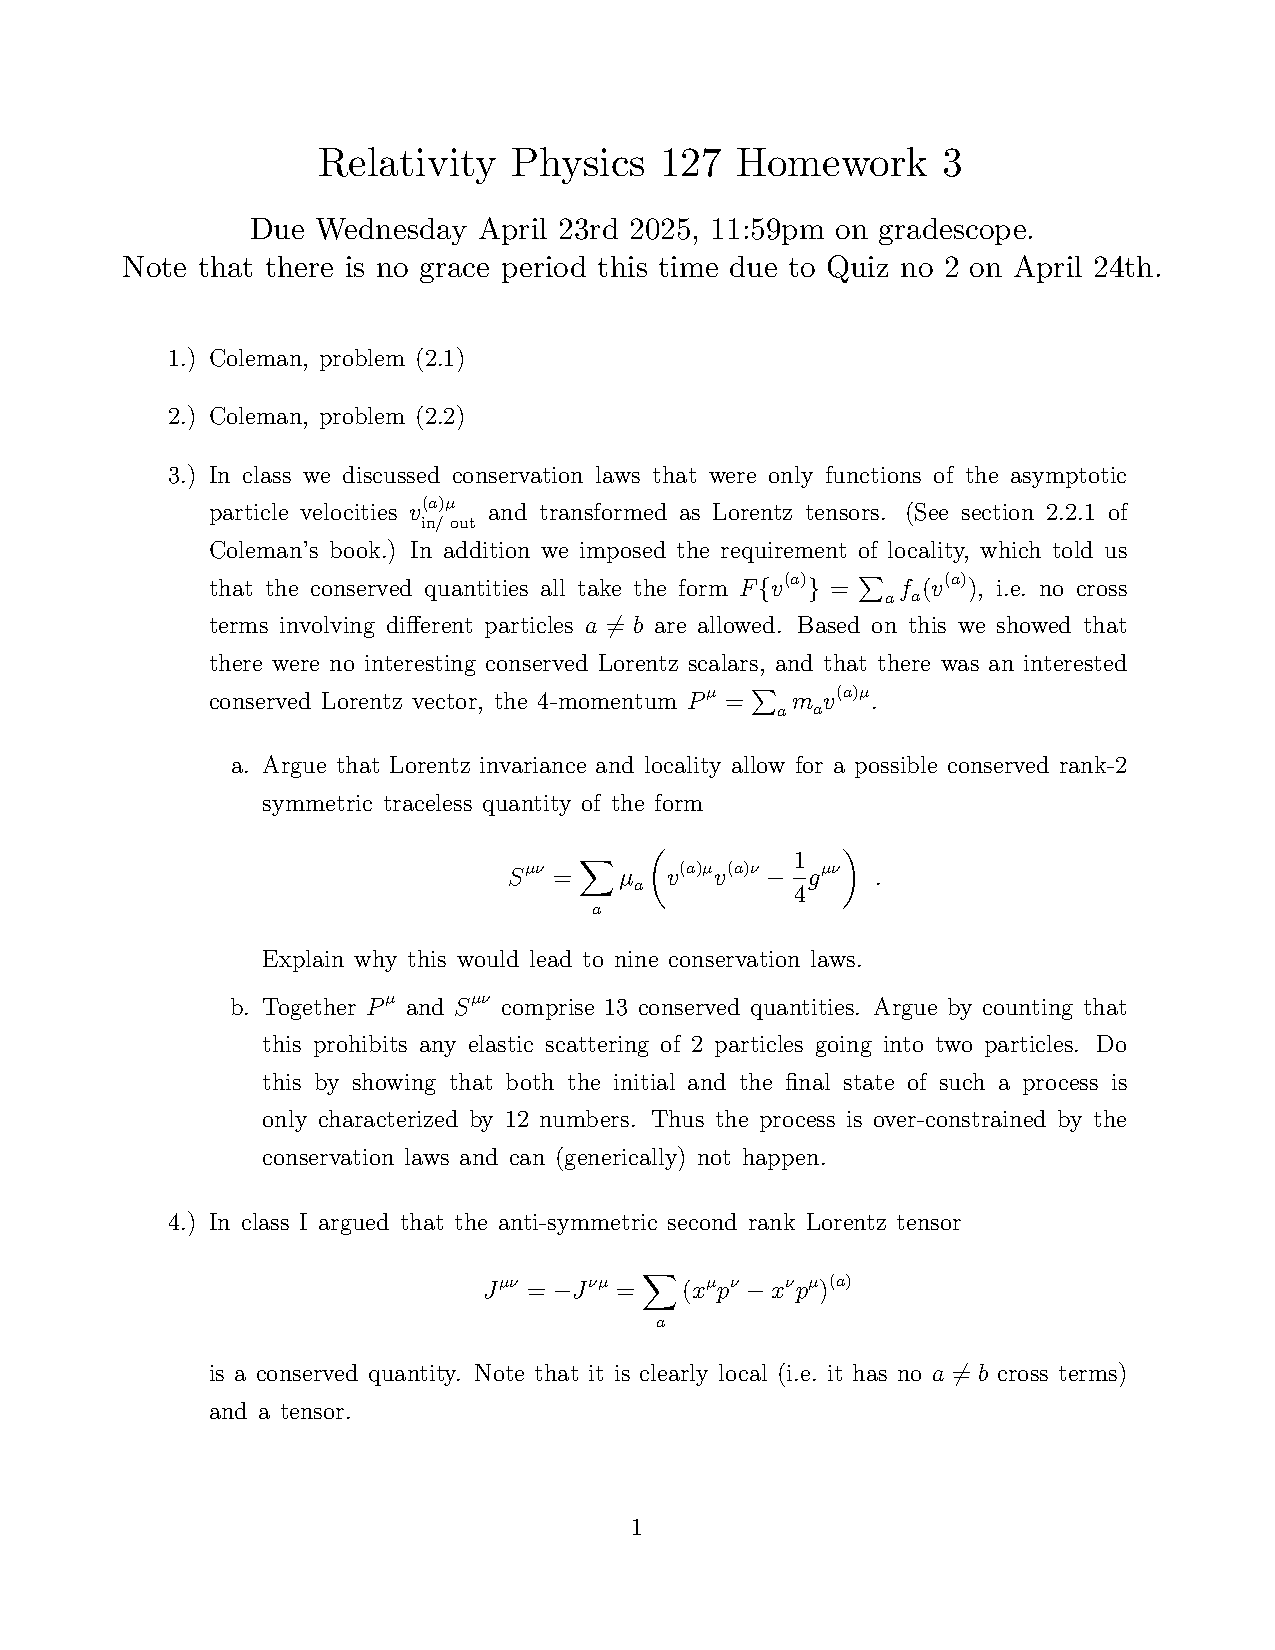
\includepdf[pages=-]{assignment.pdf}

\end{document}
